\documentclass[11pt]{article}

\usepackage[margin=1.1in]{geometry}
\usepackage{amsmath,amssymb,amsthm}
\usepackage{booktabs}
\usepackage{microtype}
\usepackage{xcolor}
\usepackage{tikz}
\usepackage{pgfplots}
\usepackage{caption}
\usepackage[hidelinks]{hyperref}

\pgfplotsset{compat=1.18}
\usetikzlibrary{arrows.meta,positioning,fit,backgrounds,calc,shapes.geometric}

% ---- palette (matched to Paper I) ----------------------------------------
\definecolor{rbred}{HTML}{B3202C}
\definecolor{rbblack}{HTML}{1A1A1A}
\definecolor{rbgrey}{HTML}{6E7278}
\definecolor{rblight}{HTML}{E8E6E1}
\definecolor{rbaccent}{HTML}{1F6F8B}

\tikzset{
  ph/.style   = {rectangle, rounded corners=3pt, draw=rbgrey, thick,
                 fill=rblight, minimum height=8mm, minimum width=20mm,
                 font=\small\sffamily, align=center},
  st/.style   = {circle, draw=rbblack, thick, fill=white,
                 minimum size=7mm, font=\scriptsize, inner sep=1pt},
  term/.style = {rectangle, draw=rbred, thick, fill=rbred!8,
                 minimum size=6mm, font=\scriptsize, inner sep=2pt},
  box/.style  = {rectangle, draw=rbaccent, thick, fill=rbaccent!6,
                 minimum height=7mm, font=\scriptsize\sffamily, align=center},
  ed/.style   = {-{Stealth[length=2mm]}, draw=rbgrey, thick},
  edr/.style  = {-{Stealth[length=2mm]}, draw=rbred, thick},
  lbl/.style  = {font=\scriptsize\sffamily, inner sep=1pt},
}

\theoremstyle{plain}
\newtheorem{theorem}{Theorem}[section]
\newtheorem{lemma}[theorem]{Lemma}
\newtheorem{corollary}[theorem]{Corollary}
\theoremstyle{definition}
\newtheorem{definition}[theorem]{Definition}
\newtheorem{example}[theorem]{Example}
\theoremstyle{remark}
\newtheorem{remark}[theorem]{Remark}

\newcommand{\R}{\ensuremath{\mathsf{R}}}
\newcommand{\B}{\ensuremath{\mathsf{B}}}
\newcommand{\rlb}{\ensuremath{r_{\mathrm{lb}}}}
\newcommand{\blb}{\ensuremath{b_{\mathrm{lb}}}}
\newcommand{\code}[1]{\texttt{\small #1}}
\newcommand{\reg}{\ensuremath{R}}
\newcommand{\infoset}{\ensuremath{I}}

\title{\bfseries The Red/Black Game II:\\[2pt]
       \large Counterfactual Regret Minimization on a Decomposed\\
       Heads-Up Game\\[4pt]
       \normalsize (Setup, Algorithm, Measurement, and the Solve)}
\author{Noah Brauner}
\date{}

\begin{document}
\maketitle
\vspace{-3.2em}

\begin{abstract}
\noindent
This paper specifies an algorithm for approximating equilibrium play in
heads-up Red/Black. It is written for a reader who has never seen
counterfactual regret minimization: Section~\ref{sec:cfr} builds CFR and
CFR+ from the definition of regret, and every later section is expressed in
those terms. The contribution is not CFR+ itself but the object it is run
on. Rather than solving the whole game at once, we cut it into one subgame
per round at the boundaries identified in Paper~I, solve each exactly, and
bootstrap upward through a layered acyclic graph of $5{,}721$ public
classes. We give a complete account of the information structure --- what an
information set is, what a player's private state consists of, and exactly
what a \emph{row} of the regret table is --- together with the vector-form
layout that makes the whole thing a sequence of dense matrix operations.
We are explicit about what the decomposition approximates: by Paper~I the
public class pins the support of the public posterior but not its shape, so
re-deriving beliefs at a boundary is a modeling choice and not an identity.
We then report the completed solve: all 5,721 classes, a game value of
51.33\% to the opening seat, and an evaluation of the resulting profile
against prior bots. The measurement sections come first because they are
what makes those numbers readable --- in particular the round-local meter
reports uniform success while seat-mirror antisymmetry, which it cannot see,
is violated by up to 0.11.
\end{abstract}

\section{Introduction}\label{sec:intro}

Paper~I described heads-up Red/Black exactly: a deterministic, acyclic
transition system whose public projection at a round boundary is two
integers per seat plus the identity of the player owing a discard. That
paper deliberately said nothing about how to play. This one does.

The target is an $\varepsilon$-equilibrium: a pair of strategies neither of
which can be improved on by much, with $\varepsilon$ measured rather than
assumed. The method is counterfactual regret minimization, in its CFR+
variant. The interesting part is not the algorithm, which is standard, but
the decomposition it runs on and the honesty of the meters attached to it.

\paragraph{Why decompose at all.}
The whole game is too large to hold in one regret table. Paper~I counted
$6{,}051$ public classes and, layer by layer, over $3\times10^{8}$
(decision node $\times$ private state) pairs. Running one CFR+ instance over
the entire game means holding all of them simultaneously and sweeping all of
them every iteration. Instead we exploit the fact --- Paper~I,
Theorem~3.7 --- that the class space is a \emph{layered directed acyclic
graph}: every round removes exactly one card, so classes at layer $T'$ can
only lead to classes at layer $T'-1$. That licenses backward induction. We
solve the smallest layer first, then use its answers as terminal payoffs for
the layer above, and so on up to the root.

\paragraph{What this buys and what it costs.}
It buys tractability: each subgame is small enough to solve to high
precision, and the layers are embarrassingly parallel within themselves.
It costs exactness. A subgame needs to know the distribution over its own
starting states, and that distribution is re-derived from the public class
rather than carried down from above. Paper~I proved (its Theorem~10.1 and
the surrounding discussion) that the public class determines the
\emph{support} of that distribution exactly but not its \emph{shape}. So the
decomposition is an approximation whose size must be measured, not argued.
Section~\ref{sec:approx} states this precisely and
Section~\ref{sec:meters} says how it is measured.

\paragraph{Scope.} Heads-up ($N=2$) throughout, hand size $H=5$, notation
continuous with Paper~I.

\paragraph{Road map.} Section~\ref{sec:recap} recaps what Paper~I
established. Section~\ref{sec:cfr} develops CFR and CFR+ from scratch.
Section~\ref{sec:info} specifies the information structure and defines a
row. Section~\ref{sec:decomp} gives the decomposition.
Section~\ref{sec:vector} gives the vector-form implementation.
Section~\ref{sec:approx} states what is approximated,
Section~\ref{sec:meters} defines the meters, and
Section~\ref{sec:results} reports the solve. Appendix~\ref{app:v1}
documents an earlier boundary choice that failed, and why.

% =========================================================================
\section{What Paper I Established}\label{sec:recap}

Four results carry over and are used without reproof.

\begin{description}\itemsep3pt
  \item[The game is a deterministic acyclic transition system.] All chance
        is in the deal; every transition is a function of state and action.
        Total cards strictly decrease, so no state recurs and every play
        terminates in between $5$ and $9$ rounds.
  \item[Two clocks.] The rules order a round \emph{reorder $\to$ bid $\to$
        procure $\to$ discard}, so the discard is last. We cut the game at
        \emph{boundaries} --- procurement resolutions, where the loser is
        known but has not yet discarded --- so the segment between two
        boundaries reads \emph{discard $\to$ reorder $\to$ bid $\to$
        procure}, with the discard first. A boundary's hand sizes $n_i$ are
        therefore \emph{pre}-discard, while the round that follows is played
        with $n_i' = n_i - [\,i=\ell\,]$ and $T' = n_0'+n_1'$. The layer
        index is $T'$.
  \item[The public class.] At a boundary the public state is
        $(\ell, s_0, s_1)$ with $s_i = (n_i, \rlb^{\,i}, \blb^{\,i})$:
        who owes a discard, each seat's pre-discard hand size, and the
        certainty bounds. There are $2K(H)^2+1 = 6{,}051$ such classes at
        $H=5$, of which $330$ are terminal and $5{,}485$ are reachable.
  \item[Knowledge is not belief.] The bounds pin the \emph{support} of the
        public posterior exactly --- sound and tight --- but say nothing
        about its shape. Two histories reaching the same class can leave an
        observer with materially different beliefs.
\end{description}

The last point is the one that constrains everything in this paper.

% =========================================================================
\section{Regret, Counterfactual Regret, and CFR+}\label{sec:cfr}

This section assumes no prior exposure. It builds the algorithm in five
steps and then states, without proving, what it guarantees.

\subsection{Regret in a one-shot game}

Suppose you play the same one-shot game repeatedly. On iteration $t$ you
choose an action $a$ from a finite set $A$, and afterwards you learn what
every action \emph{would} have paid, $u^t(a)$.

\begin{definition}[Regret]
After $T$ iterations, your \emph{cumulative regret} for action $a$ is
\[
  \reg^{T}(a) \;=\; \sum_{t=1}^{T}\Bigl(u^t(a) - u^t(\sigma^t)\Bigr),
\]
the total extra payoff you would have collected by always playing $a$
instead of what you actually played. Positive regret means $a$ was
underused.
\end{definition}

The goal is \emph{no-regret}: a rule making $\max_a \reg^{T}(a)/T \to 0$.
That is a weak-looking guarantee with a strong consequence, as we will see.

\subsection{Regret matching}

\begin{definition}[Regret matching]
Play each action with probability proportional to its positive regret so
far:
\[
  \sigma^{T+1}(a)\;=\;
  \frac{\bigl[\reg^{T}(a)\bigr]^{+}}{\sum_{a'}\bigl[\reg^{T}(a')\bigr]^{+}},
  \qquad [x]^{+}=\max(x,0),
\]
falling back to the uniform distribution when every regret is
non-positive.
\end{definition}

The intuition is exactly what it looks like: play what you wish you had
played, in proportion to how much you wish it.

\begin{example}[Worked: the keep-secret pennies]\label{ex:pennies}
Take the class in which a seat holds one certain red and one certain black
--- statistic $(2,1,1)$ --- and owes a discard. Its hand is public
knowledge; its only private decision is \emph{which card to keep}. The
opponent simultaneously decides which color to play for. Keeping the card
the opponent guesses loses; keeping the other wins. Payoffs are matching
pennies:
\[
\begin{array}{c|cc}
 & \text{opp says }\R & \text{opp says }\B\\\hline
\text{keep }\R & -1 & +1\\
\text{keep }\B & +1 & -1
\end{array}
\]
Run regret matching from zero regret. Iteration 1 is uniform, so each side
mixes $(\tfrac12,\tfrac12)$ and every action's realized value equals the
mean; regrets stay near zero and the iterates oscillate around
$(\tfrac12,\tfrac12)$ without settling on a pure action. The
\emph{average} strategy converges to $(\tfrac12,\tfrac12)$ and the game
value to $0$ --- which is the right answer, and is what the solver must
reproduce for this class.

The example also previews a practical fact: fully mixed equilibria are the
slow case for these methods. The iterates never settle, so the regret-based
convergence meter decays more slowly here than at classes with a pure or
near-pure answer.
\end{example}

\subsection{Why sequential games need something more}

Regret matching handles one decision. A round of Red/Black is a sequence of
decisions under hidden information, and two complications appear.

First, a player does not know which \emph{node} of the game tree they are
at --- only which \emph{information set} (Section~\ref{sec:info}). A
strategy must therefore be a single distribution per information set, used
at every node in it.

Second, and less obviously, you cannot just run regret matching at each
information set on its raw payoffs. The value of an information set depends
on how often play actually arrives there, which depends on the strategies
above it, including your own. Regret computed on raw payoffs mixes together
``this action is bad'' with ``I rarely get here,'' and the resulting
quantity does not decompose into something you can minimize locally.

The fix is to strip out your own contribution to arriving.

\subsection{Reach probabilities and counterfactual value}

\begin{definition}[Reach decomposition]
For a node $h$, the probability of reaching it factors into three
independent parts:
\[
  \pi(h)\;=\;\pi_{\mathrm{own}}(h)\cdot\pi_{\mathrm{opp}}(h)\cdot
             \pi_{\mathrm{chance}}(h),
\]
the contributions of the player's own choices, the opponent's choices, and
chance. Write $\pi_{-i}(h) = \pi_{\mathrm{opp}}(h)\pi_{\mathrm{chance}}(h)$
for everything \emph{except} player $i$.
\end{definition}

\begin{definition}[Counterfactual value]
The counterfactual value of information set $\infoset$ for player $i$ is
\[
  v_i(\infoset)\;=\;\sum_{h\in \infoset}\pi_{-i}(h)\; u_i(h),
\]
the expected payoff weighted by \emph{opponent-and-chance} reach only, as
if player $i$ had played to reach $\infoset$ with probability one.
\end{definition}

Dropping $\pi_{\mathrm{own}}$ is the whole trick. It makes each information
set's regret independent of how the player behaves elsewhere, so the
regrets at different information sets can be minimized separately and still
add up to a bound on the regret of the whole strategy.

\begin{definition}[Counterfactual regret; CFR]
The counterfactual regret of action $a$ at $\infoset$ is
$\reg^{T}(\infoset,a)=\sum_t \bigl(v_i^t(\infoset,a)-v_i^t(\infoset)\bigr)$,
where $v^t_i(\infoset,a)$ is the counterfactual value of playing $a$ and
then continuing with the current strategy. \emph{CFR} is: at every
information set, choose the next strategy by regret matching on
$\reg^{T}(\infoset,\cdot)$.
\end{definition}

\subsection{CFR+}

CFR+ modifies CFR in three ways. All three are practical accelerations, not
changes to what is being computed.

\begin{description}\itemsep3pt
  \item[Regret clipping.] Cumulative regrets are floored at zero after every
        update rather than allowed to go arbitrarily negative:
        $\reg^{t} \leftarrow [\reg^{t-1}+\Delta]^{+}$. An action whose
        regret has gone deeply negative would otherwise take many iterations
        to become playable again after conditions change.
  \item[Linear averaging.] The output of the algorithm is the \emph{average}
        strategy, not the current one. CFR+ weights iteration $t$ by $t$
        rather than uniformly, so late iterations --- computed from better
        regrets --- dominate.
  \item[Alternating updates.] Rather than updating both players against a
        common snapshot, update one player at a time against the other's
        current strategy.
\end{description}

\begin{remark}[The average is the answer]\label{rem:average}
This is the single most common source of confusion. The \emph{current}
strategy of a CFR run does not converge --- Example~\ref{ex:pennies} shows
it oscillating forever. The object that converges to equilibrium is the
running average. Every value, every meter, and every exported policy in
this work refers to the average strategy.
\end{remark}

\subsection{What convergence does and does not guarantee}

Regret matching gives $\max_a \reg^{T}(a) = O(\sqrt{T})$, so average regret
vanishes as $O(1/\sqrt{T})$. CFR's regret-decomposition theorem bounds a
player's total regret by the sum of counterfactual regrets over their
information sets, so minimizing locally minimizes globally. And in a
two-player zero-sum game, if both players' average regrets are at most
$\varepsilon$, the pair of average strategies is a $2\varepsilon$-equilibrium.

Three caveats matter for what follows, and each is a place where a reader
can be misled.

\begin{enumerate}\itemsep3pt
  \item \textbf{The guarantee is about average regret, not about the value
        being right.} A profile can have small regret and still sit at a
        different point of a large equilibrium set. Where the equilibrium is
        not unique --- and it is not, for the type-conditional values this
        paper bootstraps on --- two runs can converge to different, equally
        valid answers.
  \item \textbf{The guarantee is for the game you actually ran it on.} We do
        not run CFR+ on Red/Black; we run it on a decomposition of
        Red/Black (Section~\ref{sec:decomp}). Small regret in the
        decomposed game bounds exploitability \emph{in the decomposed game}.
        Transferring that claim to the real game requires a separate
        argument or, better, a separate measurement.
  \item \textbf{The bound requires perfect recall.} CFR's decomposition
        theorem assumes players never forget their own past observations or
        actions. Within a round subgame this holds. Across the boundary
        between subgames it does not, by construction: the successor is
        entered through a public class that has forgotten the bid history
        and the path by which the bounds arrived.
\end{enumerate}

Sections~\ref{sec:approx} and~\ref{sec:meters} exist because of these three
caveats.

% =========================================================================
\section{The Information Structure of a Round}\label{sec:info}

This section is the specification. It defines, in order: what a player
knows, what their private type is, what their private state is, what the
decision nodes are, and finally what a \emph{row} is.

\subsection{What a player knows}

\begin{definition}[Information set]\label{def:infoset}
Fix a class $(\ell,s_0,s_1)$ and a seat $i$. An information set of seat $i$
inside that class is a pair
\[
  \infoset \;=\; \bigl(\,\text{public node},\;\text{seat $i$'s private
  state}\,\bigr),
\]
where the \emph{public node} is everything both players can see at that
moment --- the class itself, the bid chain so far, and the flip counters
with the colors revealed this contest --- and the \emph{private state} is
everything seat $i$ knows that its opponent does not.
\end{definition}

Two seats at the same public node with different private states are at
different information sets. Two \emph{deals} that give seat $i$ the same
private state at the same public node are the \emph{same} information set:
that is precisely what seat $i$ cannot distinguish.

\subsection{Private type: $(r,x)$, and why $x$ exists}

\begin{definition}[Private type]\label{def:type}
Seat $i$'s type at a boundary is the pair
\[
  (r,\;x)\;=\;\bigl(\text{reds in its \emph{pre}-discard hand},\;
                    \text{reds among the cards it has itself discarded}\bigr).
\]
The public bounds truncate the first coordinate to
$\rlb^{\,i}\le r\le n_i-\blb^{\,i}$; the second is invisible to the
opponent.
\end{definition}

The first coordinate is unsurprising. The second deserves explanation,
because it is easy to mistake for bookkeeping.

Discarded cards are out of play and can never be flipped, so $x$ cannot
affect any payoff directly. It is nonetheless \emph{payoff-relevant
information}, because the deck is finite. There are exactly $26$ red and
$26$ black cards. A seat that has seen many reds among its own cards ---
in hand or discarded --- knows the unseen remainder is red-poor, and can
price its opponent's hand accordingly. Concretely, a player who has seen
$k$ reds among their own five dealt cards should assign an unseen card
probability $(26-k)/47$ of being red, which ranges from $0.447$ to $0.553$
as $k$ runs from $5$ to $0$.

So $x$ is private information about the \emph{deck}, not about the hand.
Under an idealized infinite deck it would carry no information and could be
dropped, collapsing the type space to $r$ alone. It is retained because the
real game is played with $52$ cards.

\subsection{Private states: what a seat actually chooses}

A type is a piece of knowledge; a \emph{private state} is a concrete
realization the seat acts from. The two differ because a seat gets to
choose its hand order, and the pending loser additionally chooses what to
drop.

\begin{definition}[Private state]\label{def:privstate}
For a seat that is \textbf{not} the pending discarder, a private state is
\[
  \bigl(\text{an ordering of its } (r,\,n_i-r) \text{ color multiset},\;x\bigr),
\]
one per admissible ordering, of which there are $\binom{n_i}{r}$.

For the \textbf{pending discarder}, the drop and the reorder are a single
joint private choice, so a private state is
\[
  \bigl(\text{drop color}\;\times\;\text{ordering of the surviving }
  n_i-1 \text{ cards},\;x'\bigr),
\]
where $x'=x+1$ if the dropped card was red and $x'=x$ otherwise. Two paths
that reach the same post-discard hand --- dropping a red from $r$ reds
versus dropping a black from $r-1$ --- remain \emph{distinct} states,
because they imply different $x'$ and therefore different beliefs about
the deck.
\end{definition}

\begin{remark}[Why the drop and the reorder are joint]
Separating them would let the reorder condition on a drop the opponent
never sees, which is exactly the information leak the boundary placement
exists to prevent. Treating them as one choice keeps the keep-secret
decision and every response to it inside a single exactly-solved game.
\end{remark}

\begin{example}[Counting private states]\label{ex:states}
Take the class $\ell=0$, $s_0=(2,0,0)$, $s_1=(1,0,0)$ --- seat $0$ owes a
discard from two cards, nothing is publicly certain about either hand.

\emph{Seat $0$}, the discarder, has $n_0=2$ so it has made $H-n_0=3$
discards, giving $x\in\{0,1,2,3\}$; with no bounds, $r\in\{0,1,2\}$. That is
$3\times4=12$ types. Its joint (drop, ordering) choices per $r$ are:
$r=0$ must drop black, leaving \B{} --- $1$ choice; $r=1$ may drop either,
leaving \B{} or \R{} --- $2$; $r=2$ must drop red, leaving \R{} --- $1$.
Hence
\[
  \text{states}_0 \;=\; (1+2+1)\times 4 \;=\; \mathbf{16}.
\]

\emph{Seat $1$} has $n_1=1$, so $4$ discards and $x\in\{0,\dots,4\}$, and
$r\in\{0,1\}$: $2\times5=10$ types, each with exactly one ordering of a
single card. Hence $\text{states}_1=\mathbf{10}$.
\end{example}

\subsection{Decision nodes}

Within a round, the public structure is the round automaton of Paper~I,
built on the \emph{in-round} sizes $(n_0',n_1')$. Two kinds of node carry
decisions:

\begin{description}\itemsep2pt
  \item[Bid nodes] $(\text{color},\,\text{chain})$, plus the pre-bid node.
        There are $2^{\,T'+1}-1$ of them. The actor alternates with chain
        length.
  \item[Procurement nodes] $(\text{color},\,\text{chain},\,x,\,y)$ where
        $x,y$ count cards already flipped off the bidder's and challenger's
        decks. Only the bidder acts. By Paper~I's order-irrelevance lemma
        these form a lattice on the two counters, not a tree of flip
        sequences.
\end{description}

Resolutions are terminal within the round; they do not carry decisions,
they carry values (Section~\ref{sec:decomp}).

\subsection{Rows}\label{sec:rows}

\begin{definition}[Row]\label{def:row}
A \emph{row} is one (decision node, private state) pair belonging to the
seat that acts at that node. Each row holds a cumulative-regret vector and
a cumulative-strategy vector, one entry per legal action. The row count is
the size of the regret table and the primary determinant of both memory and
time.
\end{definition}

The count is \emph{not} a simple product of nodes and states, for two
reasons: different nodes are acted on by different seats, and procurement
nodes are masked by consistency --- a bidder whose flipped prefix would not
have matched the bid color cannot be at that node at all, so that row does
not exist.

\begin{example}[Rows, continued from Example~\ref{ex:states}]\label{ex:rows}
Same class. The starter is $1-\ell = 1$, and the in-round sizes are
$(1,1)$, so the round graph has $7$ bid nodes and $14$ procurement nodes.

Of the $7$ bid nodes, seat $1$ acts at $3$ and seat $0$ at $4$:
\[
  \text{rows}_{\text{bid}} \;=\; 3\times 10 \;+\; 4\times 16 \;=\; 94 .
\]
Of the $14$ procurement nodes, seat $1$ is the bidder at $8$ and seat $0$
at $6$, which would give $8\times10+6\times16=176$ rows unmasked. The
consistency mask removes $26$, leaving
$\text{rows}_{\text{proc}}=150$. In total
\[
  \text{rows} \;=\; 94+150 \;=\; \mathbf{244}.
\]
\end{example}

Table~\ref{tab:rowscale} gives the totals by layer. They are structural ---
derivable without solving anything --- and they are what a run must budget
for.

\begin{remark}[A lossless reduction the present solver does not take]
\label{rem:orderclass}
Those counts enumerate hand orderings in full, and they need not. Paper~I
shows that an ordering's observable content is exactly its \emph{leading
run}: a hand opening with $k$ cards of color $a$ can never reveal anything
at position $k+2$ or beyond, because procurement halts at that seat's first
off-color card under either bid color, flipping removes no cards, and the
next round reorders anyway. So orderings agreeing on
$(a,k)$ are indistinguishable in every continuation, and the
$\binom{r+b}{r}$ orderings of an $(r,b)$ multiset collapse to
$r+b$ classes (one, if the hand is monochrome).

This is \emph{lossless} --- unlike the belief abstraction of
Section~\ref{sec:approx}, nothing is approximated --- but the
implementation described here does not exploit it: \code{build\_privates}
enumerates raw orderings. Taking it would remove about $12\%$ of private
states outright and, because the saving grows with depth ($0\%$ at
$T'\le4$, $15\%$ at $T'=8$, $24\%$ at $T'=9$, $31\%$ at the root) while the
deep layers hold most of the rows, roughly $\mathbf{19\%}$ of the total row
count in Table~\ref{tab:rowscale} --- some $62$M of $336$M, with $T'=9$
alone contributing $40$M.

Two caveats on the size. It requires $n\ge4$ to appear at all, since
$\binom{n}{r}=r+b$ for $n\le3$; and it is capped at $50\%$ per composition,
so lopsided hands ($r\in\{0,1,n-1,n\}$) save nothing. It is therefore not
transformative alone. Its real value is that it partially funds a
refinement that \emph{costs} space: if a future version enriches the public
statistic to make concealment visible (Section~\ref{sec:approx}), this
claws back a fifth of the bill.
\end{remark}

\begin{table}[htbp]
\centering
\caption{Regret-table size by layer. ``Classes'' counts those with a real
subgame; terminal classes hold a value and no rows. The distribution is
extremely top-heavy: layers $8$ and $9$ hold $81.5\%$ of all rows. The root
($T'=10$) is the whole game and yet costs less than a percent --- see
Remark~\ref{rem:rootcheap}.}
\label{tab:rowscale}
\begin{tabular}{@{}lrrrr@{}}
\toprule
Layer $T'$ & Classes & Rows & Mean rows/class & Share\\
\midrule
$2$ & $36$ & $5{,}424$ & $150$ & $0.002\%$\\
$3$ & $132$ & $70{,}056$ & $530$ & $0.021\%$\\
$4$ & $330$ & $546{,}656$ & $1{,}656$ & $0.163\%$\\
$5$ & $686$ & $3{,}181{,}392$ & $4{,}637$ & $0.948\%$\\
$6$ & $1{,}104$ & $13{,}760{,}056$ & $12{,}463$ & $4.100\%$\\
$7$ & $1{,}290$ & $43{,}581{,}784$ & $33{,}784$ & $12.985\%$\\
$8$ & $1{,}260$ & $106{,}941{,}312$ & $84{,}874$ & $31.862\%$\\
$9$ & $882$ & $166{,}740{,}672$ & $189{,}048$ & $49.678\%$\\
$10$ (root) & $1$ & $815{,}456$ & $815{,}456$ & $0.243\%$\\
\midrule
all & $5{,}721$ & $335{,}642{,}808$ & & \\
\bottomrule
\end{tabular}
\end{table}

\begin{remark}[The root is the biggest game and one of the cheapest classes]
\label{rem:rootcheap}
The root is the full $5$-versus-$5$ game. Its \emph{public} structure is the
largest anywhere --- $2{,}047$ bid nodes and $65{,}790$ procurement nodes,
more than any other class --- and yet it holds only $815{,}456$ rows, about
four average layer-$9$ classes.

The reason is that rows are the product of public nodes and \emph{private
states}, and at the root the private side is at its smallest. Nobody has
discarded yet, so $x=0$ for both seats and the type space collapses from
$(r,x)$ to $r$ alone: $6$ types per seat, and $\sum_r \binom{5}{r} = 2^5 =
32$ private states. Contrast a layer-$9$ class, where each seat has made
discards, $x$ ranges over several values, and the private state count is
multiplied accordingly.

This inverts the naive intuition that the game gets cheaper as it gets
smaller. It does not: the public game shrinks with $T'$, but the private
state space \emph{grows} with the number of discards, and the second effect
dominates. The expensive layers are the middle-to-late ones, where hands are
still large enough for many orderings and enough cards have been discarded
for $x$ to range widely.
\end{remark}

\subsection{Entry beliefs}\label{sec:entrybeliefs}

A subgame cannot be solved without a distribution over the type pairs it
starts from. We use the \emph{bounded hypergeometric} law: treat both hands
as drawn from the residual $26/26$ budget and renormalize over the region
the public bounds allow.

This is the one modeling choice in the design, and Section~\ref{sec:approx}
is about its consequences. Note what it is not: it is not the exact
posterior, because the exact posterior depends on how the opponent has been
playing.

% =========================================================================
\section{Decomposition}\label{sec:decomp}

\subsection{Subgames}

\begin{definition}[Round subgame]\label{def:subgame}
The subgame rooted at a non-terminal class $(\ell,s_0,s_1)$ consists of:
the pending discarder's joint (drop, reorder) choice; the other seat's
reorder; the bidding phase; and procurement, ending at the resolution
\emph{before} the next discard.
\end{definition}

Two boundary cases. \emph{Terminal} classes --- those whose pending
discarder holds a single card --- have no subgame at all: the forced discard
eliminates that seat and the value is $\pm1$. The \emph{root} is the
opposite special case: $\ell=-1$, so no discard is pending, the pre-stage is
just the two reorders, and the bidding starter is seat $0$ by convention
rather than $1-\ell$. Everything downstream of the pre-stage is identical.

\subsection{Backward induction over layers}

Every resolution of a subgame at layer $T'$ identifies a successor class at
layer $T'-1$: apply the realized discard's decay to the entry bounds, raise
them to the colors seen this round, and record the new loser. Because $T'$
strictly decreases, the classes form a layered DAG and can be solved
bottom-up.

\begin{figure}[htbp]
\centering
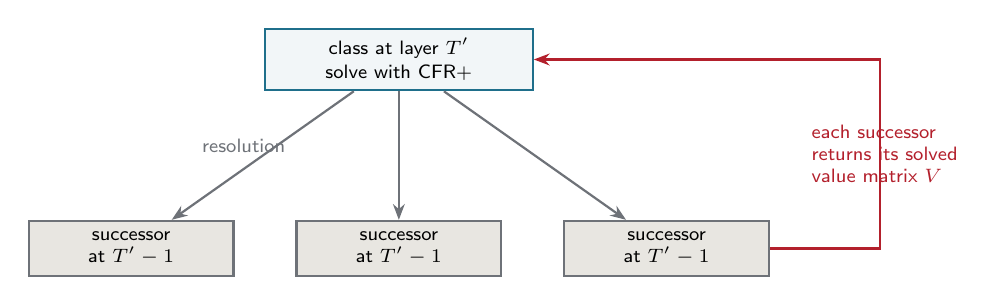
\begin{tikzpicture}[x=1mm,y=1mm]
  \node[box, minimum width=34mm] (par) at (0,0)
    {class at layer $T'$\\[1pt]\scriptsize solve with CFR+};
  \node[box, minimum width=26mm, fill=rblight, draw=rbgrey] (c1) at (-34,-24)
    {successor\\at $T'-1$};
  \node[box, minimum width=26mm, fill=rblight, draw=rbgrey] (c2) at (0,-24)
    {successor\\at $T'-1$};
  \node[box, minimum width=26mm, fill=rblight, draw=rbgrey] (c3) at (34,-24)
    {successor\\at $T'-1$};
  \foreach \c in {c1,c2,c3}{ \draw[ed] (par) -- (\c); }
  \node[lbl, text=rbgrey, anchor=east] at (-14,-11) {resolution};
  % single return path, routed clear of every box
  \draw[edr] (c3.east) -- ++(14,0) |- (par.east);
  \node[lbl, text=rbred, anchor=west, align=left] at (52,-12)
    {each successor\\returns its solved\\value matrix $V$};
\end{tikzpicture}
\caption{One step of the recursion. A class is solved with CFR+ over its own
round; its terminal payoffs are type-conditional values returned by
already-solved successors one layer down.}
\label{fig:recursion}
\end{figure}

\subsection{Bootstrapping}

\begin{definition}[Type-conditional value matrix]\label{def:vtypes}
Write $m_i$ for the number of seat $i$'s types. The solution of a class
returns a matrix $V\in\mathbb{R}^{m_0\times m_1}$, where $V[t_0,t_1]$ is the
seat-$0$ value when the seats hold types $t_0,t_1$ and both play the solved
average strategy.
\end{definition}

A parent's resolution looks up its successor class and reads off the entry
of $V$ matching the types the seats hold at that moment. Only $V$ is needed
to solve a parent, which is why high layers can be solved against a
values-only store rather than full child solutions.

\begin{remark}[$V$ is not unique]\label{rem:vnotunique}
Different equilibria of the same subgame can produce different $V$ while
agreeing on the aggregate value. Where a private coordinate is
payoff-irrelevant but belief-relevant --- $x$ is exactly this --- the
solver may split a mixed strategy into near-pure branches indexed by that
coordinate, and the individual entries of $V$ are then arbitrary across the
equilibrium set. The aggregate is pinned; the cells are not. This is a
measurement trap, and Section~\ref{sec:meters} returns to it.
\end{remark}

% =========================================================================
\section{Vector-Form CFR+}\label{sec:vector}

\subsection{Why not walk information sets}

The textbook presentation of CFR walks the game tree recursively, visiting
one node at a time. That is a poor fit here. The number of private states
per seat is large and their structure is identical --- every private state
of a seat faces the same public node with the same legal actions. Walking
them individually means millions of tiny scalar operations.

Instead we hold, at each public node, a \emph{matrix} whose rows are the
acting seat's private states and whose columns are the legal actions. An
iteration then becomes a sequence of dense matrix operations over public
nodes, with the private dimension vectorized.

\subsection{Layout}

Per class, for each seat $i$:

\begin{center}\small
\begin{tabular}{@{}lll@{}}
\toprule
Object & Shape & Meaning\\
\midrule
\code{states} & $P_i$ & private states (Definition~\ref{def:privstate})\\
\code{type\_idx} & $P_i$ & which type each private state belongs to\\
\code{regret[node]} & $P_i \times A_{\text{node}}$ & cumulative regret, one row per state\\
\code{strat\_sum[node]} & $P_i \times A_{\text{node}}$ & cumulative strategy, linearly weighted\\
\code{reach} & $P_i$ & current reach for each private state\\
\code{entry\_wt} & $|\text{types}_0|\times|\text{types}_1|$ & bounded-hypergeometric prior\\
\bottomrule
\end{tabular}
\end{center}

The row count of Definition~\ref{def:row} is exactly
$\sum_{\text{nodes}} P_{\text{actor(node)}}$, restricted by the consistency
masks --- which is what Example~\ref{ex:rows} computed by hand.

\subsection{Consistency masks}

A private state is not compatible with every public node. If a procurement
node records that three cards came off a seat's deck and all matched the
bid color, then any private state whose top three cards are not all that
color is impossible there. Rather than branch, we precompute a boolean mask
per (node, seat) and zero the corresponding rows. Masked rows are excluded
from the row count because they can never be reached.

\subsection{One sweep}

An iteration, for the player being updated:

\begin{enumerate}\itemsep2pt
  \item \textbf{Strategy.} At each node, regret-match the regret matrix
        rowwise to get a strategy matrix, clipping negatives (CFR+).
  \item \textbf{Forward.} Propagate reach from the entry weights through the
        pre-stage choice and then down the public graph, multiplying by the
        acting seat's strategy and applying masks.
  \item \textbf{Backward.} Compute counterfactual values at resolutions by
        contracting the successor's value matrix $V$ against the opponent's
        reach, then propagate upward, accumulating per-action values.
  \item \textbf{Regret.} Add (action value $-$ node value), weighted by
        opponent-and-chance reach, into the regret matrix; clip at zero.
  \item \textbf{Average.} Accumulate $t\cdot\pi_{\mathrm{own}}\cdot\sigma$
        into the strategy sum.
\end{enumerate}

Then swap players. The average strategy is recovered by normalizing
\code{strat\_sum} rowwise.

\begin{remark}[Averaging must not be gated by opponent reach]
The accumulation in step~5 must run at every information set the updating
player can reach on their own, regardless of whether the opponent currently
reaches it. Gating on opponent reach freezes rows the opponent has
temporarily stopped visiting, leaving early garbage in the average and
making the result spuriously exploitable.
\end{remark}

\subsection{Cost model}

Time per class scales as
\[
  \text{cost}\;\approx\;\frac{\text{rows}\times\text{iterations}}
                             {\text{throughput}},
\]
with throughput in row-iterations per second. Rows are structural
(Table~\ref{tab:rowscale}); iterations are what convergence demands and are
reported in the companion paper. The important structural fact is the
top-heaviness: half the total row count lives at layer $9$ alone, and
layers $8$ and $9$ together are $81.5\%$ of the work. Any scheduling decision
should be made about those two layers first.

% =========================================================================
\section{What Is Approximated}\label{sec:approx}

The algorithm above solves each subgame essentially exactly. The
approximation lives entirely in how subgames are joined.

\subsection{The belief reset}

To solve a subgame we need a distribution over its starting type pairs. We
re-derive it from the public class using the bounded-hypergeometric law of
Section~\ref{sec:entrybeliefs}. We do \emph{not} carry down the posterior
that the actual history would have induced.

Paper~I makes precise what that discards. Its Theorem~10.1 shows the class
determines the support of the public posterior exactly --- the certainty
bounds are sound and tight. But the shape of the distribution on that
support is not determined: two histories reaching the same class can leave
an observer with materially different beliefs, because the bound-folding
rule remembers a bound's height while forgetting whether it is fresh
evidence or the decayed residue of a taller one. Cross-round bid history is
discarded outright.

\subsection{Consequences}

\begin{enumerate}\itemsep3pt
  \item \textbf{The solved profile is an equilibrium of a different game.}
        Call it $G'$: Red/Black with beliefs reset to the class prior at
        every boundary. CFR+'s guarantees apply to $G'$. In the real game
        the profile is a candidate strategy whose exploitability must be
        measured.
  \item \textbf{Round-local convergence cannot certify the composition.}
        A class can be solved to arbitrarily small round-local
        exploitability while the values it inherited from below are drawn
        from a different point of a non-unique equilibrium set
        (Remark~\ref{rem:vnotunique}).
  \item \textbf{The error is not automatically small.} Appendix~\ref{app:v1}
        documents a boundary placement that produced a $9.5$ percentage
        point error on a concrete position while remaining internally
        consistent by every round-local measure. That case motivated the
        present boundary; it is not evidence that the current one is exact.
\end{enumerate}

None of this is an argument against decomposing. It is an argument for
measuring, which is the next section.

% =========================================================================
\section{Measurement}\label{sec:meters}

Three instruments, three different claims. Confusing them is the main way
to overstate a result.

\subsection{Round-local exploitability}

\begin{definition}[$\varepsilon_{\text{round}}$]
For a single class, hold the solved continuation values fixed and compute
both players' exact best responses against the average profile \emph{within
that round}. The sum of their gains is the round-local exploitability.
\end{definition}

\textbf{Certifies:} that CFR+ has converged on this subgame, given its
inherited values. \textbf{Does not certify:} anything about composition.
It is computed with the successor values held fixed, so it is blind by
construction to whether those values were right.

\subsection{Composed exploitability}

\begin{definition}[$\varepsilon_{\text{comp}}$]
Best-respond across the whole class DAG --- in the round and in every
successor round --- against the cached average profile.
\end{definition}

\textbf{Certifies:} exploitability in $G'$, the belief-reset game.
\textbf{Does not certify:} exploitability in Red/Black. Two sub-meters are
worth distinguishing: a \emph{lower bound}, obtained because any concrete
deviating strategy's gain bounds the true best response from below; and an
\emph{exact} figure for a redeal variant in which types are re-drawn at
every boundary, where scalar continuations make backward induction exact.
Neither removes the belief reset --- they measure inside it.

\subsection{The perfect-recall oracle}

\begin{definition}[Oracle bracket]
Build the explicit perfect-recall game tree over the raw engine, with
information sets indexed by a player's full own history and every public
observation, so nothing the real game remembers is forgotten. Then bracket
the value with exact best responses.
\end{definition}

\textbf{Certifies:} the true value, in the real game, with no belief reset
anywhere. \textbf{Limitation:} the tree is built explicitly, so this is
restricted to small classes. It is the only instrument here that speaks
about Red/Black rather than about $G'$, and it is the one that scales
worst --- a combination worth stating plainly rather than burying.

\subsection{Summary}

\begin{table}[htbp]
\centering
\caption{What each instrument certifies. No single row is sufficient, and
the rightmost column is the one that matters for any claim about the real
game.}
\label{tab:meters}
\begin{tabular}{@{}llll@{}}
\toprule
Instrument & Scope & Certifies about & Scales?\\
\midrule
$\varepsilon_{\text{round}}$ & one class & convergence, given inherited values & yes\\
$\varepsilon_{\text{comp}}$ & class DAG & exploitability in $G'$ & yes\\
Oracle bracket & one small class & the true value in Red/Black & no\\
Seat mirror & class pair & internal consistency & yes\\
\bottomrule
\end{tabular}
\end{table}

The seat mirror deserves a note. A class and its seat-swapped image must
have exactly opposite values, for any correct solver. At layers where a
subgame is the entire remaining game the mirror is tight; once classes
bootstrap from other classes, mirror discrepancy becomes a cheap proxy for
composition error --- precisely the quantity $\varepsilon_{\text{round}}$
cannot see. It is the only instrument in the table that is both scalable
and sensitive to composition, which makes it the practical tripwire for a
large run.

\subsection{What would constitute a defensible claim}

Not ``the game is solved.'' The defensible form is a conjunction: a stated
round-local tolerance across all classes; a composed exploitability in
$G'$; an oracle agreement on the small classes where it can be computed;
mirror consistency as a function of depth; and an explicit statement that
the profile is an equilibrium of $G'$ rather than of Red/Black. The
companion paper reports these.

\section{Results}\label{sec:results}

The game has been solved: all $5{,}721$ classes, every layer from $T'=2$ to
the root.

\subsection{The solve}

\begin{table}[htbp]
\centering
\caption{Convergence by layer at $\mathrm{tol}=10^{-3}$,
$\mathrm{max\_iters}=6000$. Every class in every layer converged; no class
hit the cap.}
\label{tab:convergence}
\begin{tabular}{@{}lrrrrr@{}}
\toprule
Layer $T'$ & Classes & Median iters & Max iters & Max $\varepsilon_{\text{round}}$ & Rows\\
\midrule
$2$  & $36$      & $275$ & $3{,}075$ & $9.9\times10^{-4}$ & $5{,}424$\\
$3$  & $132$     & $200$ & $2{,}075$ & $9.9\times10^{-4}$ & $70{,}056$\\
$4$  & $330$     & $125$ & $1{,}850$ & $1.0\times10^{-3}$ & $546{,}656$\\
$5$  & $686$     & $100$ & $1{,}575$ & $1.0\times10^{-3}$ & $3{,}181{,}392$\\
$6$  & $1{,}104$ & $150$ & $1{,}475$ & $1.0\times10^{-3}$ & $13{,}760{,}056$\\
$7$  & $1{,}290$ & $200$ & $1{,}025$ & $1.0\times10^{-3}$ & $43{,}581{,}784$\\
$8$  & $1{,}260$ & $250$ & $900$     & $1.0\times10^{-3}$ & $106{,}941{,}312$\\
$9$  & $882$     & $350$ & $975$     & $1.0\times10^{-3}$ & $166{,}740{,}672$\\
$10$ & $1$       & $475$ & $475$     & $9.8\times10^{-4}$ & $815{,}456$\\
\midrule
all & $5{,}721$ & & & & $335{,}642{,}808$\\
\bottomrule
\end{tabular}
\end{table}

Layers $2$ through $9$ ran on a 28-physical-core cloud VM in $43{,}653$\,s
($12.1$ hours) for about \$23; the root ran locally in $2{,}019$\,s
($33.6$ minutes). The root is one class, so it cannot be parallelized and
core \emph{speed} is all that matters --- an Apple M-series performance core
measured $\approx\!2.2\times$ a cloud core here, which is why bringing a
single class home beat leaving it on the fleet.

Two practical findings. First, $\mathrm{max\_iters}$ must be generous:
fully mixed classes --- the keep-secret matching-pennies shape of
Example~\ref{ex:pennies} --- need $\sim\!2{,}700$ iterations against a
median of a few hundred, and the common default of $800$ silently truncates
about $17\%$ of the shallowest layer, failing the $\varepsilon$ gate for
reasons that have nothing to do with the game. A high cap is nearly free
because the solver exits at tolerance.

Second, median iterations are \textbf{U-shaped} in depth: $275$ at $T'=2$,
falling to $100$ at $T'=5$, then climbing to $350$ at $T'=9$ and $475$ at
the root. Extrapolating a cost model from the shallow layers alone reads the
descending arm and underestimates the deep ones.

\subsection{The value of the game}

\[
  v(\text{root}) \;=\; +0.0266 \quad\Longrightarrow\quad
  \mathbf{51.33\%} \text{ to the player who opens.}
\]

So the opening seat holds an edge of about $1.3$ percentage points. That sits
between the two small games solved by hand in Paper~I --- $51.92\%$ at
$T'=2$ and $52.83\%$ at the four-card root --- and it should be read with
the caveat of Section~\ref{sec:resmeters}: to about $\pm0.1$, not to the
digit.

\subsection{What the meters say}\label{sec:resmeters}

Every class converged: $\varepsilon_{\text{round}} \le 10^{-3}$ everywhere,
with no class hitting the iteration cap. On the round-local meter the solve
is uniformly green.

That meter is not the story. Seat-mirror antisymmetry must hold
\emph{exactly} --- $v(\ell{=}0,A,B) = -v(\ell{=}1,B,A)$ --- and over all
$5{,}720$ mirror pairs it does not:

\begin{center}\small
\begin{tabular}{@{}lrrrrrrrr@{}}
\toprule
Layer $T'$ & $2$ & $3$ & $4$ & $5$ & $6$ & $7$ & $8$ & $9$\\
\midrule
Worst gap & $0.0002$ & $0.0056$ & $0.0141$ & $0.0288$ & $0.1142$ & $0.0767$ & $0.0495$ & $\mathbf{0.1146}$\\
\bottomrule
\end{tabular}
\end{center}

Median $0.0014$; worst $0.1146$, which is over $100\times$ that class's own
$\varepsilon_{\text{round}}$ and $5.7$ percentage points of win rate. This is
exactly the failure Section~\ref{sec:meters} predicted:
$\varepsilon_{\text{round}}$ certifies a class against its inherited values
and is blind by construction to whether those values were right.

Two features of that table deserve emphasis. The gap does \emph{not} decay
with depth --- it is bimodal, peaking at $T'=6$ and again at $T'=9$. And
$T'=9$, the worst layer in the entire solve, is the layer every game enters
on its second round. The best-calibrated numbers are the ones a player sees
last.

\subsection{Playing the profile}

The solved profile was mapped into the game engine and evaluated over
paired games (each deal played from both seats):

\begin{center}\small
\begin{tabular}{@{}lrrr@{}}
\toprule
Opponent & Win rate & Wilson 95\% CI & Games\\
\midrule
gen6 CFR (previous best) & $78.85\%$ & $[77.56,\,80.09]$ & $4{,}000$\\
Heuristic & $87.10\%$ & $[86.03,\,88.10]$ & $4{,}000$\\
Random & $99.88\%$ & $[99.71,\,99.95]$ & $4{,}000$\\
\bottomrule
\end{tabular}
\end{center}

Across $283{,}793$ decisions the profile drove \emph{every} decision:
zero fallbacks, zero out-of-range positions, zero on-demand solves. Since a
misplaced boundary or a pre- versus in-round size confusion surfaces as a
fallback, that is meaningful evidence the class mapping is correct, and all
$15{,}643$ joint discard-and-reorder commitments replayed exactly.

The sharpest check is self-play, which closes the loop between the solved
number and the running game:
\[
  \text{measured seat-0 rate } 0.5100,\ \text{95\% CI } [0.4881,\,0.5319]
  \quad\text{vs solved } 0.5133 .
\]
The solved value falls inside the interval. Table, mapping and engine agree.
The residual, $-0.0033$, has the sign the theory predicts --- a profile
optimal in $G'$ gives up a little when played in Red/Black --- though it is
far inside the interval and so not established.

\subsection{What is not established}

Three limits, stated plainly.

\textbf{The win rates do not measure distance from equilibrium.} Neither
gen6 nor the heuristic probes the abstraction, so neither can detect a
$0.11$ mirror gap or the concealment blindness below. Beating them shows the
table is sound and playable; it says nothing about exactness.

\textbf{The raw profile is not safe alone.} With the play-time guards
disabled, self-play logged $1{,}024$ suicide flips in $28{,}368$
procurement decisions and $294$ impossible bids in $28{,}211$. With guards
on, both are zero. The guard layer is not cosmetic: the unguarded policy
makes locally losing plays, concentrated exactly where value flows through
the successor bootstrap.

\textbf{One strategic defect is identified and reproducible.} In a $3$-vs-$5$
round the profile flips its \emph{own} deck with probability one while
holding a single black against an opponent certainly holding three. Both
flip orders have identical win probability, and flipping the opponent's
weakly dominates, because it preserves the option of never revealing your
own card. The solver cannot see this: the decision has \emph{zero}
round-local payoff difference, so all of its value sits in successor values,
and it acted on a $0.033$ margin where the measured error at that layer is
$0.0495$. Sampled over $12.0$M two-way procurement rows, $92.6\%$ of such
decisions are genuinely mixed and only $3.9\%$ pure --- but $42.1\%$ of the
pure ones rest on margins inside the noise floor. CFR+ goes pure whenever
values differ at all, so solver noise is laundered into confident advice.

All three trace to Section~\ref{sec:approx}: beliefs re-derived at each
boundary from a statistic that Paper~I proves is support-complete but not
distribution-complete. Closing them is a redesign, not a tuning exercise.

\appendix

\section{An Earlier Boundary, and Why It Failed}\label{app:v1}

The boundary of Definition~\ref{def:subgame} places the pending discard at
the \emph{start} of a subgame. An earlier design placed it at the
\emph{end} --- subgames ran reorder $\to$ bid $\to$ procure $\to$ discard,
matching the rules' own phrasing. That choice is more natural to write down
and it is wrong, in a way worth recording because the failure was invisible
to every round-local check.

\paragraph{The counterexample.} Consider a seat holding one card, known to
be red, first to act, against a seat holding a known red and a known black.
By a two-stage matching-pennies argument the true value of this position is
exactly $25\%$ to the first seat. The end-of-round decomposition priced it
at $15.5\%$.

\paragraph{The mechanism.} With the discard at the end of a subgame, the
loser's keep-secret decision falls in one subgame while every response to
it falls in the next. The successor was solved standalone against a class
prior, which committed it to near-pure responses conditioned on the
opponent's type. The parent's discard could then choose the card that beats
that already-frozen book --- an exploit the real game forbids, because the
response cannot be conditioned on a secret it has not seen. The keep-secret
and the response are simultaneous in the real game, and the boundary had
severed them.

\paragraph{Why it was invisible.} Round-local exploitability was small.
Composed best-response brackets confirmed the $15.5\%$ tightly --- but
\emph{within the belief-reset game}, which is what
Section~\ref{sec:meters} warns about. The number was internally consistent
and externally wrong. Only an oracle that refused the belief reset could
see it.

\paragraph{The fix.} Move the boundary one discard earlier, so that the
keep-secret decision and every response to it live inside a single exactly
solved subgame. That is Definition~\ref{def:subgame}, and it is why the
pending discarder's drop and reorder are a joint private choice
(Definition~\ref{def:privstate}).

\paragraph{The lesson, stated generally.} A decomposition boundary must
never cut a coupling between moves that the real game makes at the same
time. Where it does, each side gets solved against a frozen model of the
other, and the error can be large while every meter computed inside the
decomposition reports success.

\section{Notation}\label{app:notation}

Continuous with Paper~I; new symbols marked $\dagger$.

\begin{center}\small
\begin{tabular}{@{}ll@{}}
\toprule
Symbol & Meaning\\
\midrule
$H$ & hand size at the deal; $H=5$\\
$n_i,\;T$ & hand size / cards in play at a boundary (\emph{pre}-discard)\\
$n_i',\;T'$ & hand size / cards in play during the round; $T'$ is the layer index\\
$\ell$ & seat owing a discard; $-1$ at the root\\
$s_i=(n_i,\rlb^{\,i},\blb^{\,i})$ & seat $i$'s public statistic\\
$(r,x)$ & private type: reds held, reds among own discards\\
$P_i$ $\dagger$ & number of seat $i$'s private states\\
$\infoset$ $\dagger$ & information set\\
$\reg^T(\infoset,a)$ $\dagger$ & cumulative counterfactual regret\\
$\pi_{\mathrm{own}},\pi_{\mathrm{opp}},\pi_{-i}$ $\dagger$ & reach probabilities\\
$v_i(\infoset)$ $\dagger$ & counterfactual value\\
$V$ $\dagger$ & type-conditional value matrix of a solved class\\
$G'$ $\dagger$ & the belief-reset game the solver actually solves\\
$\varepsilon_{\text{round}},\varepsilon_{\text{comp}}$ $\dagger$ & round-local / composed exploitability\\
\bottomrule
\end{tabular}
\end{center}

\end{document}
